\section{Conclusions}

To address the change of its scope from electron to pion identification for momenta greater than 3.5~GeV,
the original CLAS Cherenkov Counters were refurbished at part of the new CLAS12 Low Threshold Cherenkov
Counter (LTCC) system. The work included improvements of the reflectivities for the mirrors and the Winston
cones, p-terphenyl coating of the PMTs, expansion of the gas volumes, and redesign of the box walls and patch
panels. The LTCC detector sectors after refurbishment are shown in \F{ltccInstalled} installed on the CLAS12
Forward Carriage upstream of the Forward Time-of-Flight system. The average LTCC efficiency for electron
detection in the momentum range from 3.5 to 6.5~GeV is 94\%. The pion efficiency starts around 50\% near
the expected signal threshold, and rises with momentum as expected. A plateau of 88\% is reached at a momentum
of 5~GeV. This is within range of an expectation of efficiency above 90\%. Additional future studies are required
to full quantify the detection efficiency of the CLAS12 LTCC for both positive and negative pions as a function of
momentum.

\begin{figure}
    \centering
    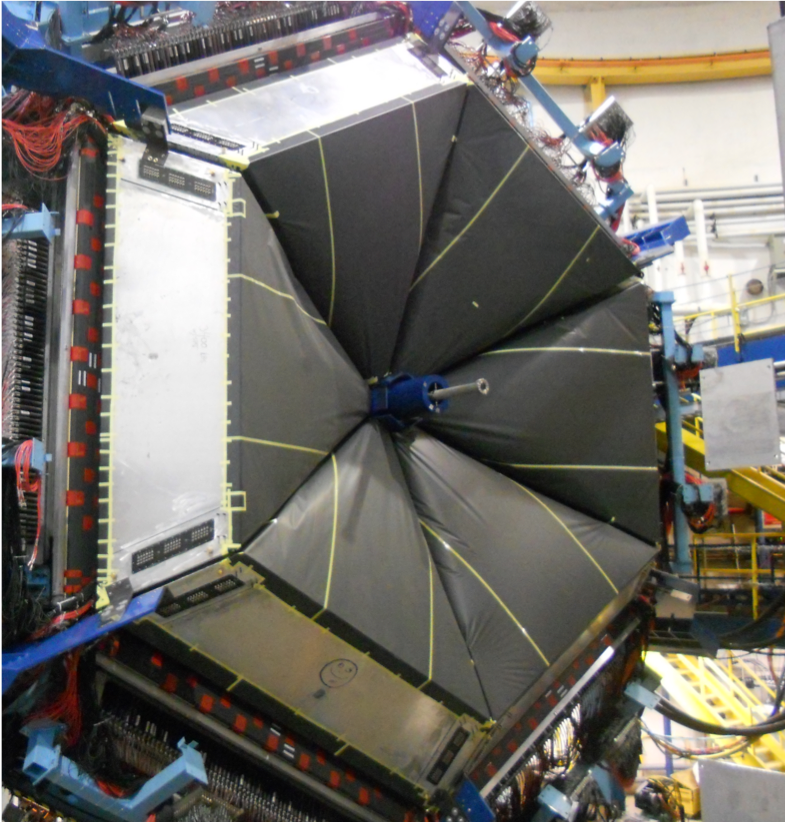
\includegraphics[width=1.0\columnwidth,keepaspectratio]{img/ltccInstalled.png}
    \caption{The LTCC sectors installed after refurbishment on the CLAS12 Forward Carriage. The RICH detector
    is installed in the sector~4 position and the sector~1 position awaits the installation of a second RICH detector.}
    \label{fig:ltccInstalled}
\end{figure}

\section{Acknowledgments}

We thank the Detector Support Group at Jefferson Lab for the work on the cone refurbishment, reflectivity tests,
PMT divider modifications and installation, and for designing the gas control system and associated software. We
thank Temple University for the p-terphenyl deposition. We thank Vladimir Popov for the implementation of the
divider base modification. We thank Youri Sharabian and Steve Christo for their consultations and contributions.
We thank the technical team of Hall~B for their work and dedication on all aspect of the project. Finally, we thank
all the Hall~B staff for their unyielding support. This work was supported in part by
DOE Contract DE-AC05-84ER40150.
